\documentclass[11pt]{article}

\usepackage[utf8]{inputenc}
\usepackage[T1]{fontenc}
\usepackage[a4paper,margin=1in]{geometry}
\usepackage{xcolor}
\usepackage{graphicx}
\usepackage{booktabs}
\usepackage{array}
\usepackage{longtable}
\usepackage{enumitem}
\usepackage{listings}
\usepackage{fancyhdr}
\usepackage{titlesec}
\usepackage{tikz}
\usetikzlibrary{positioning,arrows.meta,fit,backgrounds}
\usepackage[hidelinks]{hyperref}

% ---- palette ----
\definecolor{acnavy}{HTML}{1F2A44}
\definecolor{acblue}{HTML}{2D6CDF}
\definecolor{acteal}{HTML}{0E7C7B}
\definecolor{acgray}{HTML}{5B6472}
\definecolor{aclight}{HTML}{EEF2F8}
\definecolor{acred}{HTML}{C0392B}
\definecolor{acamber}{HTML}{B9770E}
\definecolor{acgreen}{HTML}{1E8449}
\definecolor{accode}{HTML}{F4F6FB}

\hypersetup{colorlinks=true,linkcolor=acblue,urlcolor=acblue}

% ---- headers/footers ----
\pagestyle{fancy}
\fancyhf{}
\renewcommand{\headrulewidth}{0.4pt}
\lhead{\textcolor{acgray}{\small Achernar — End-to-End Wiring Audit}}
\rhead{\textcolor{acgray}{\small\thepage}}
\lfoot{\textcolor{acgray}{\small Confidential — Internal Engineering}}

% ---- section styling ----
\titleformat{\section}{\Large\bfseries\color{acnavy}}{\thesection}{0.6em}{}
\titleformat{\subsection}{\large\bfseries\color{acblue}}{\thesubsection}{0.6em}{}
\titleformat{\subsubsection}{\normalsize\bfseries\color{acteal}}{\thesubsubsection}{0.6em}{}

% ---- listings ----
\lstset{
  basicstyle=\ttfamily\footnotesize,
  backgroundcolor=\color{accode},
  breaklines=true,
  frame=single,
  rulecolor=\color{aclight},
  framesep=6pt,
  xleftmargin=4pt,
  xrightmargin=4pt,
  columns=fullflexible,
  keepspaces=true,
  showstringspaces=false,
}

% severity tags
\newcommand{\sev}[1]{\textbf{\textcolor{acred}{#1}}}
\newcommand{\sevm}[1]{\textbf{\textcolor{acamber}{#1}}}
\newcommand{\sevl}[1]{\textbf{\textcolor{acgray}{#1}}}
\newcommand{\ok}[1]{\textbf{\textcolor{acgreen}{#1}}}
\newcommand{\fn}[1]{\texttt{#1}}

\newcommand{\statusbadge}[2]{\colorbox{#1}{\textcolor{white}{\bfseries\,#2\,}}}

\begin{document}

% ============================= TITLE =============================
\begin{titlepage}
\centering
\vspace*{1.4cm}
{\color{acnavy}\rule{\linewidth}{1.4pt}}\\[0.5cm]
{\Huge\bfseries\color{acnavy} Achernar}\\[0.35cm]
{\LARGE\color{acblue} End-to-End Wiring Audit, Fixes \& Roadmap}\\[0.4cm]
{\large\color{acgray} Unified Astronomy Imaging and Control System}\\[0.3cm]
{\color{acnavy}\rule{\linewidth}{1.4pt}}\\[1.0cm]

\begin{tabular}{rl}
\textbf{Scope} & Daemon $\leftrightarrow$ Backend $\leftrightarrow$ Frontend $\leftrightarrow$ Desktop wiring \\[2pt]
\textbf{Repository} & \texttt{Achernar.tech} (monorepo) \\[2pt]
\textbf{Reference spec} & \texttt{achernar\_v4} (System Architecture, rev.\ Mar 2026) \\[2pt]
\textbf{Prepared for} & Ibrahim Shahid, Lead Architect \\[2pt]
\textbf{Date} & June 13, 2026 \\[2pt]
\textbf{Document type} & Engineering audit + change record \\
\end{tabular}

\vfill
{\color{acgray}\small This report documents the current state of the four-tier system,
the end-to-end wiring fixes applied in this engineering pass, the verification performed,
and a prioritized roadmap toward a working application.}
\vspace*{1cm}
\end{titlepage}

\tableofcontents
\newpage

% ============================= 1. EXEC SUMMARY =============================
\section{Executive Summary}

Achernar is a four-tier system for controlling astronomy imaging equipment. The repository
is substantially more mature than a prototype: all four tiers exist, the hardware-access core
compiles to a binary, and the architecture closely tracks the \texttt{achernar\_v4} specification.
The dominant problems are not missing components --- they are \emph{wiring} defects: places where
two tiers were independently correct but could not reliably talk to each other, and an unfinished
refactor that left the frontend with two competing copies of its API layer.

This pass focused on the \textbf{end-to-end wiring} between the tiers. We mapped every
inter-tier connection (HTTP routes, WebSocket channels, the cloud reverse-tunnel relay, and the
runtime transport switch), audited build/health status, and corrected five concrete defects ---
including two that silently break the system only in production or only on a fresh clone, which is
exactly the class of bug that is most expensive to discover later.

\begin{table}[h]
\centering
\renewcommand{\arraystretch}{1.3}
\begin{tabular}{>{\raggedright\arraybackslash}p{0.40\linewidth} >{\raggedright\arraybackslash}p{0.16\linewidth} >{\raggedright\arraybackslash}p{0.34\linewidth}}
\toprule
\textbf{Tier} & \textbf{Status} & \textbf{Headline} \\
\midrule
Rust daemon + C/C++ FFI bridge & \ok{Healthy} & Compiles to binary; FFI surface is sound \\
Django backend (17 apps) & \ok{Healthy} & Relay correct after cache fix \\
React/TS web frontend & \ok{Healthy} & Split-brain API layer consolidated \\
Tauri desktop shell & \sevm{Partial} & Sidecar mgr solid; dev wiring fixed \\
OpenLiveStacker drivers / SDKs & \sevm{Bloated} & Vendored twice ($\approx$9.6\,GB) \\
\bottomrule
\end{tabular}
\caption{Per-tier status at the end of this pass.}
\end{table}

\noindent\textbf{Five fixes shipped this pass} (Section~\ref{sec:fixes}): (1) a Redis-backed cache so the
command relay survives multi-process deployment; (2) consolidation of the duplicated frontend API/env/hooks
layers; (3) a \texttt{.gitignore} correction so the frontend's transport-switch code is actually tracked;
(4) a Tauri \texttt{beforeDevCommand} so the desktop hosts the real web app in development; and (5) product
naming/title cleanup. All changes were verified (Section~\ref{sec:verify}).

% ============================= 2. ARCHITECTURE =============================
\section{System Architecture}

\subsection{The four tiers}

\begin{itemize}[leftmargin=1.2em]
  \item \textbf{Daemon} (\fn{achernar-daemon}, Rust, $\approx$5{,}800 LOC across 11 subsystems): the
  on-site edge service. Exposes an HTTP+WebSocket API on \texttt{127.0.0.1:3030} and talks to hardware
  through a C/C++ FFI bridge into the OpenLiveStacker (OLS) drivers and vendor SDKs.
  \item \textbf{Backend} (\fn{backend}, Django 4.2 + DRF + Channels, $\approx$2{,}500 LOC, 17 apps):
  the cloud control plane. Hosts the REST API the browser calls and the WebSocket ``gateway'' the daemon
  dials into (the IoT reverse tunnel).
  \item \textbf{Frontend} (\fn{achernar-frontend}, React 18 + TypeScript + Vite, $\approx$1{,}600 LOC):
  the operator UI. At runtime it chooses one of two transports --- direct-to-daemon (desktop) or
  via the Django relay (browser).
  \item \textbf{Desktop} (\fn{achernar-desktop}, Tauri 2, $\approx$285 LOC Rust): a thin shell that
  \emph{hosts the web frontend} and \emph{manages the daemon as a sidecar} (launch / health-check / stop).
\end{itemize}

\subsection{End-to-end data flow}

\begin{figure}[h]
\centering
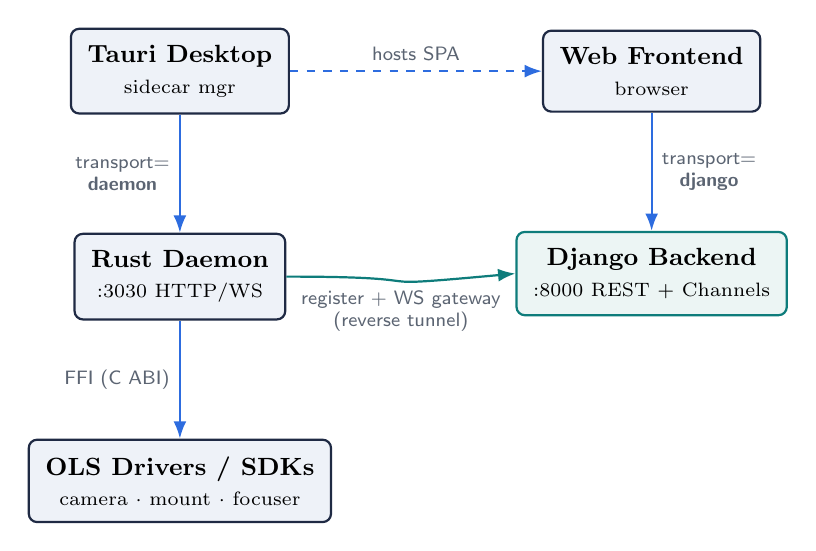
\begin{tikzpicture}[
  font=\small,
  box/.style={rounded corners=3pt,draw=acnavy,thick,fill=aclight,align=center,minimum height=1.0cm,inner sep=6pt},
  cloud/.style={rounded corners=3pt,draw=acteal,thick,fill=acteal!8,align=center,minimum height=1.0cm,inner sep=6pt},
  edge/.style={-{Latex[length=2.2mm]},acblue,thick},
  lbl/.style={font=\scriptsize\sffamily,acgray,align=center}
]
% nodes
\node[box] (desktop) {\textbf{Tauri Desktop}\\\scriptsize sidecar mgr};
\node[box,below=1.5cm of desktop] (daemon) {\textbf{Rust Daemon}\\\scriptsize :3030 HTTP/WS};
\node[box,right=3.2cm of desktop] (browser) {\textbf{Web Frontend}\\\scriptsize browser};
\node[cloud,below=1.5cm of browser] (django) {\textbf{Django Backend}\\\scriptsize :8000 REST + Channels};
\node[box,below=1.5cm of daemon] (hw) {\textbf{OLS Drivers / SDKs}\\\scriptsize camera $\cdot$ mount $\cdot$ focuser};

% desktop hosts frontend (both render the same SPA)
\draw[edge,dashed] (desktop) -- node[lbl,above]{hosts SPA}(browser);

% desktop transport: direct to daemon
\draw[edge] (desktop.south) -- node[lbl,left]{transport=\\\textbf{daemon}}(daemon.north);

% browser transport: via django
\draw[edge] (browser.south) -- node[lbl,right]{transport=\\\textbf{django}}(django.north);

% daemon reverse tunnel up to django
\draw[edge,acteal] (daemon.east) .. controls +(2.2,0) and +(-2.2,-0.2) .. node[lbl,below,pos=0.5]{register + WS gateway\\(reverse tunnel)}(django.west);

% daemon to hardware
\draw[edge] (daemon.south) -- node[lbl,left]{FFI (C ABI)}(hw.north);
\end{tikzpicture}
\caption{Two operator paths converge on one daemon. In the desktop, the frontend detects the Tauri
runtime and talks \emph{directly} to the local daemon; in the browser it talks to Django, which relays
commands to the daemon over a daemon-initiated WebSocket ``gateway.''}
\label{fig:flow}
\end{figure}

\noindent The crucial design idea (Figure~\ref{fig:flow}) is the \textbf{runtime transport switch}
(\fn{src/lib/runtime.ts}): \texttt{getHardwareTransport()} returns \texttt{"daemon"} inside Tauri and
\texttt{"django"} in a browser. Every data hook keys off this, so the same React code drives both the
desktop (LAN-local, low latency) and the browser (internet, via relay).

% ============================= 3. PER-TIER AUDIT =============================
\section{Per-Tier Audit}

\subsection{Daemon and the C/C++ FFI bridge}

The hardware-access core is the part you specifically asked to validate, and it is in good shape.
The Rust source is organised into the subsystems the spec calls for:

\begin{lstlisting}
ai/  api/  control/  filter_wheel/  focus/  hardware/
models/  mount/  processing/  storage/  vision/
control/{control_supervisor, action_arbiter, safety_guard, ownership}.rs
focus/{focus_agent, focus_inference, focus_policy, backlash, ...}.rs
\end{lstlisting}

\noindent\textbf{FFI appropriateness (your headers).} The bridge is a clean three-layer design:

\begin{enumerate}[leftmargin=1.4em]
  \item \fn{ols-bridge/include/ols\_bridge.h} --- a \emph{flat C ABI} (opaque handles +
  integer error codes) wrapping the OLS C++ classes. This is the correct boundary: a stable
  \texttt{extern "C"} surface is what Rust can bind to safely.
  \item \fn{src/hardware/ols\_ffi.rs} --- Rust \texttt{extern} declarations that map 1:1 to the header,
  with \texttt{\#[repr(C)]} structs for frames, formats and parameters.
  \item \fn{ols-bridge/src/ols\_bridge.cpp} --- the implementation, compiling OLS driver sources directly
  and replacing the heavy \texttt{cppcms}/\texttt{booster} dependencies with header-only shims
  (\texttt{nlohmann/json} + minimal socket wrappers).
\end{enumerate}

\noindent The C symbol surface covers camera (sim / Alpaca / ASI / SVBony / Touptek), mount (Alpaca),
and focuser (Alpaca) with create / list / open / parameter / stream entry points, and \fn{build.rs}
drives the CMake build and links the result. \textbf{Evidence it compiles:} both
\fn{target/debug/achernar-daemon} and \fn{target/release/achernar-daemon} are present as built binaries.
We did not force a full \texttt{cargo} rebuild in this pass (it is heavy --- LTO plus $\approx$428 C++
translation units plus an ONNX Runtime download) and we made \emph{no} Rust changes, so the existing
binaries remain valid.

\begin{table}[h]
\centering
\renewcommand{\arraystretch}{1.25}
\begin{tabular}{>{\raggedright\arraybackslash}p{0.30\linewidth} >{\raggedright\arraybackslash}p{0.62\linewidth}}
\toprule
\textbf{Daemon HTTP/WS route} & \textbf{Purpose} \\
\midrule
\texttt{GET /health} & Liveness (used by the Tauri sidecar manager) \\
\texttt{GET /api/v1/status} & Aggregate camera/mount/focuser state \\
\texttt{POST /api/v1/connect} & Connect equipment by \texttt{\{type, driver, option\}} \\
\texttt{POST /api/v1/camera/stream/start} & Begin live view \\
\texttt{GET /api/v1/camera/stream} (WS) & Binary frame packets \\
\texttt{POST /api/v1/mount/*} & slew / sync / park / tracking / abort \\
\texttt{POST /api/v1/focuser/*} & move / moveto / position / abort \\
\texttt{GET /ws/telemetry} (WS) & 1\,Hz telemetry stream \\
\bottomrule
\end{tabular}
\caption{Daemon API surface actually mounted in \fn{main.rs}.}
\end{table}

\noindent\textbf{Gaps (roadmap, not wiring):} \fn{api/focus.rs} defines the spec's autofocus control
endpoints (\texttt{/api/v1/focus/*}) but every handler is a \texttt{todo!()} stub; they are correctly
\emph{not} mounted (mounting panicking stubs would be worse). The frontend's \texttt{analyze()} helper
points at \texttt{/api/v1/ai/analyze}, which the daemon does not serve; it is unused by the live UI.

\subsection{Backend (Django control plane)}

Seventeen apps, ASGI-first (\texttt{daphne} is the first installed app), Channels for WebSockets, DRF for
REST. The reverse-tunnel relay is implemented end-to-end: \fn{apps/sync/views.py} registers daemons,
\fn{apps/realtime/consumers.py} runs the \texttt{DaemonConsumer} (gateway) and \texttt{TelemetryConsumer}
(browser fan-out), and \fn{apps/equipment/views.py} turns a browser REST call into a relayed command and
waits for the result. Dev/prod settings are cleanly split; dev falls back to SQLite + in-memory Channels,
prod mandates Postgres + Redis. The one real defect here (the cache handoff) is detailed in
Section~\ref{sec:fixes}.

\subsection{Frontend (React/TypeScript)}

Feature-organised (\texttt{cloud, filter, focus, imaging, mount, session, settings}) with a clean
\texttt{api / hooks / pages / stores / types} split and React Query for data. The transport switch is the
right abstraction. The defect was an \textbf{unfinished \texttt{src/} $\rightarrow$ \texttt{src/lib/}
migration} that left two divergent copies of the API client, the env config, and two hooks --- with
\fn{Dashboard.tsx} importing from \emph{both}. Consolidated this pass (Section~\ref{sec:fixes}).

\subsection{Desktop (Tauri shell)}

The Rust side is the highlight: \fn{src-tauri/src/lib.rs} is a genuine \texttt{DaemonManager} that locates
the daemon binary, launches it as a child process, performs a raw-socket health check, forwards cloud
env vars, and tears the process down on exit. Configuration already points the bundled app at the real
web frontend (\texttt{frontendDist}) and builds it (\texttt{beforeBuildCommand}). What was missing was the
\emph{development} counterpart --- nothing started the frontend dev server --- plus leftover scaffold
(the default ``Tauri + React'' greet page) that is dead because the shell hosts the frontend, not its own
\texttt{src/}.

% ============================= 4. WIRING ANALYSIS =============================
\section{End-to-End Wiring Analysis}

\subsection{Browser path (transport = django)}
\begin{lstlisting}
Browser  --HTTP-->  Django /api/equipment/command/  (send_relay_command)
         channel_layer.group_send -> DaemonConsumer (WS) -> daemon
daemon executes -> COMMAND_RESULT -> DaemonConsumer -> cache.set(result)
Django view polls cache.get(result)  ----> HTTP response to browser
\end{lstlisting}
This loop is correct \emph{provided the WS consumer and the HTTP view share one cache} --- the subject of
Fix~1.

\subsection{Desktop path (transport = daemon)}
\begin{lstlisting}
Tauri launches -> DaemonManager.start() spawns achernar-daemon (:3030)
Webview loads frontend -> getHardwareTransport()=="daemon"
Frontend --HTTP/WS--> daemon directly (status, stream, commands)
\end{lstlisting}
Correct, and now complete in dev once Fix~4 starts the frontend server that the webview points at.

\subsection{Daemon reverse tunnel (cloud relay)}
\begin{lstlisting}
daemon -> POST {ACHERNAR_CLOUD_HTTP}/api/sync/register/  (X-Achernar-Relay-Token)
       <- { daemon_id, gateway_url }
daemon -> WS {ACHERNAR_CLOUD_WS}/ws/gateway/{daemon_id}/?token=...
       -> HELLO / HEARTBEAT(10s) / TELEMETRY(1s)
       <- COMMAND ; -> COMMAND_RESULT
\end{lstlisting}
URL normalization on both ends matches (trailing-slash handling, \texttt{/api} and \texttt{/ws} prefixes).
Token check is symmetric (\texttt{ACHERNAR\_RELAY\_DEV\_TOKEN}).

% ============================= 5. ISSUES & FIXES =============================
\section{Issues Found and Fixes Implemented}\label{sec:fixes}

\begin{longtable}{>{\raggedright\arraybackslash}p{0.05\linewidth} >{\raggedright\arraybackslash}p{0.08\linewidth} >{\raggedright\arraybackslash}p{0.49\linewidth} >{\raggedright\arraybackslash}p{0.22\linewidth}}
\toprule
\textbf{\#} & \textbf{Sev.} & \textbf{Issue} & \textbf{Disposition} \\
\midrule
\endhead
1 & \sev{High} & \texttt{CACHES} never defined; relay result handoff rides default per-process LocMemCache --- breaks under multi-process/scaled ASGI & \ok{Fixed} \\
2 & \sev{High} & Frontend split-brain: duplicate \texttt{src/api} vs \texttt{src/lib/api}, two env + two hooks; \texttt{Dashboard} imported both & \ok{Fixed} \\
3 & \sev{High} & \texttt{.gitignore} \texttt{lib/} excludes \texttt{achernar-frontend/src/lib} --- transport switch untracked, breaks fresh clone/CI & \ok{Fixed} \\
4 & \sevm{Med} & Tauri \texttt{dev} had no \texttt{beforeDevCommand}; webview pointed at an unstarted :5173 & \ok{Fixed} \\
5 & \sevl{Low} & Generic product naming (window/title ``Tauri + React'') & \ok{Fixed} \\
6 & \sevm{Med} & OLS drivers vendored twice ($\approx$9.6\,GB committed) & \textit{Roadmap} \\
7 & \sevl{Low} & \texttt{/api/v1/focus/*} stubs; \texttt{ai/analyze} dead helper; \texttt{config.rs} unused by \texttt{main.rs} & \textit{Roadmap} \\
\bottomrule
\caption{Issue register. Items 1--5 were corrected and verified this pass.}
\end{longtable}

\subsection{Fix 1 --- Cache backend for the relay handoff (\sev{High})}
\fn{backend/settings/base.py}. The browser command path depends on the ASGI WebSocket consumer and the
synchronous DRF view exchanging a result through \texttt{django.core.cache}. With the default LocMemCache
this works for a single process but \emph{silently} fails when more than one process/replica runs (the
polling worker never sees the writing worker's result; every command returns ``pending''). We back the
cache with Redis whenever \texttt{REDIS\_URL} is set, mirroring the existing \texttt{CHANNEL\_LAYERS} logic.

\begin{lstlisting}
if os.getenv('REDIS_URL'):
    CACHES = {'default': {
        'BACKEND': 'django.core.cache.backends.redis.RedisCache',
        'LOCATION': os.getenv('REDIS_URL')}}
else:
    CACHES = {'default': {
        'BACKEND': 'django.core.cache.backends.locmem.LocMemCache',
        'LOCATION': 'achernar-relay'}}
\end{lstlisting}

\subsection{Fix 2 --- Consolidate the frontend API layer (\sev{High})}
We made the top-level \texttt{src/} canonical and kept the \emph{better} implementation of each duplicated
module: the superset \fn{src/api/daemon.ts} (with \texttt{relayCommand}, \texttt{cameraStreamWsUrl},
\texttt{startCameraStream}) and the \emph{transport-aware} \fn{src/hooks/useTelemetrySocket.ts} (which skips
the direct daemon socket in browser mode instead of throwing). Imports in \fn{MjpegLiveView.tsx} and
\fn{Dashboard.tsx} were repointed off \texttt{../lib/...}, and the stale \fn{src/lib/api},
\fn{src/lib/env.ts}, \fn{src/lib/hooks} were deleted. \fn{src/lib/runtime.ts} remains as the single shared
util. No live caller used the methods that differed between the copies, so behaviour is preserved.

\subsection{Fix 3 --- Track the frontend \texttt{src/lib} directory (\sev{High})}
\fn{.gitignore}. The Python-oriented \texttt{lib/} pattern matched \fn{achernar-frontend/src/lib}, so the
transport-switch code was never committed --- it builds on the author's machine but is absent from a clean
clone. Added scoped negations:
\begin{lstlisting}
!achernar-frontend/src/lib/
!achernar-frontend/src/lib/**
\end{lstlisting}
\texttt{node\_modules/**/lib} remains correctly ignored.

\subsection{Fix 4 --- Tauri hosts the web app in development (\sevm{Med})}
\fn{src-tauri/tauri.conf.json}. Added \texttt{"beforeDevCommand": "pnpm --dir ../achernar-frontend dev"}
so \texttt{tauri dev} boots the real frontend on :5173 (which \texttt{devUrl} already targets). With the
existing sidecar manager, the desktop now starts the daemon, serves the frontend, and the frontend detects
Tauri and talks to the daemon directly --- a complete local loop.

\subsection{Fix 5 --- Product naming (\sevl{Low})}
Window title and \fn{index.html} title set to ``Achernar'' (from the default ``Tauri + React'').

% ============================= 6. VERIFICATION =============================
\section{Verification}\label{sec:verify}

\begin{table}[h]
\centering
\renewcommand{\arraystretch}{1.3}
\begin{tabular}{>{\raggedright\arraybackslash}p{0.34\linewidth} >{\raggedright\arraybackslash}p{0.58\linewidth}}
\toprule
\textbf{Check} & \textbf{Result} \\
\midrule
Frontend typecheck & \ok{Pass} --- \texttt{tsc --noEmit -p tsconfig.app.json} exits 0 under \texttt{strict}, \texttt{noUnusedLocals} \\
Backend cache config & \ok{Pass} --- both backend dotted paths import in Django 4.2.9; LocMem branch round-trips set/get \\
Settings syntax & \ok{Pass} --- \texttt{py\_compile} on base/dev/prod \\
Tauri config & \ok{Pass} --- \texttt{tauri.conf.json} parses as valid JSON \\
\texttt{.gitignore} fix & \ok{Pass} --- \texttt{git status} now lists \texttt{src/lib/} as trackable; \texttt{node\_modules} lib still ignored \\
Daemon build & \ok{Prior} --- debug+release binaries present; no Rust changed this pass \\
\bottomrule
\end{tabular}
\caption{Verification performed this pass.}
\end{table}

\noindent\textbf{Not yet run (deferred, see roadmap):} a full \texttt{cargo build} of the daemon (heavy
C++/ONNX toolchain), a Django \texttt{manage.py check} against the real virtualenv (the committed venv
targets host Python 3.14, unavailable in the audit sandbox), and a live three-process smoke test.

% ============================= 7. ROADMAP =============================
\section{Roadmap to a Working App}

\subsection*{Phase 1 --- Make it run end-to-end locally (days)}
\begin{itemize}[leftmargin=1.3em]
  \item Add \fn{achernar-frontend/.env} with \texttt{VITE\_DAEMON\_URL}, \texttt{VITE\_CLOUD\_API},
  \texttt{VITE\_DAEMON\_WS}; document \texttt{VITE\_HARDWARE\_TRANSPORT} override.
  \item Smoke-test both loops: \texttt{start\_local.sh} (browser$\rightarrow$Django$\rightarrow$daemon relay)
  and \texttt{pnpm tauri dev} (desktop$\rightarrow$daemon direct), using the \texttt{sim} camera driver.
  \item Decide the \texttt{ai/analyze} contract: implement \texttt{/api/v1/ai/analyze} in the daemon or
  remove the dead frontend helper.
  \item Wire \fn{main.rs} to \texttt{AchernarConfig::load()} so \fn{achernar.toml} actually configures the
  daemon (today only env vars are read).
\end{itemize}

\subsection*{Phase 2 --- Repository hygiene (days)}
\begin{itemize}[leftmargin=1.3em]
  \item De-duplicate OpenLiveStacker: keep one vendored copy (git submodule \emph{or} a single tracked
  tree) and reference it from the daemon; move large binaries to Git LFS. This reclaims $\approx$4.8\,GB
  and removes drift between the two copies.
  \item Remove the dead Tauri scaffold (\fn{src/App.jsx}, \fn{main.jsx}, \fn{assets/react.svg}) now that
  the shell hosts the frontend.
  \item Add CI: \texttt{tsc}, \texttt{cargo check} (daemon + desktop), \texttt{manage.py check}. This would
  have caught Fixes 1--3 automatically.
\end{itemize}

\subsection*{Phase 3 --- Spec features (weeks)}
\begin{itemize}[leftmargin=1.3em]
  \item Implement the autofocus control loop behind \texttt{/api/v1/focus/*}
  (\texttt{control\_supervisor} $\rightarrow$ \texttt{action\_arbiter} $\rightarrow$ \texttt{safety\_guard}
  $\rightarrow$ \texttt{focus\_agent}).
  \item Ship the edge ONNX models (FQE / COC / TED / background-SNR) and load them via the model registry.
  \item Implement session-frame upload (\texttt{apps/sync/upload-session} is a 501 stub) and the telemetry
  ``digital twin'' snapshot history.
\end{itemize}

\subsection*{Phase 4 --- Hardening for production (weeks)}
\begin{itemize}[leftmargin=1.3em]
  \item Replace the shared dev relay token + \texttt{AllowAny} equipment endpoints with real per-user auth
  and per-daemon ownership.
  \item Set a real CSP (currently \texttt{null}), enable prod security settings, and add observability
  (structured logs, health/metrics) across all tiers.
\end{itemize}

\vspace{0.6cm}
\begin{center}
{\color{acnavy}\rule{0.5\linewidth}{0.8pt}}\\[4pt]
{\small\color{acgray} End of report --- Achernar end-to-end wiring audit, June 13, 2026.}
\end{center}

\end{document}
